\chapter{OBJECT RECONSTRUCTION AND SAMPLE SELECTION}
\label{sec:EventReconstruction}

For each event that passes the trigger, the output from all of the sub-detectors described in Chapter~\ref{chap:Detector} is saved by the data acquisition system (DAQ) and eventually recorded to disk and tape. The data format at this stage is referred to as ``RAW" data. It includes information about the response of each detector, but the data are still unprocessed, aside from the minimal processing done to determine whether the event passed the trigger. ``Reconstruction" is the general term for algorithms that convert the detector response data into lists of object candidates---muons, photons, electrons, jets, etc.---and event quantities such as missing transverse momentum \ETmiss.

Figure~\ref{fig:cmsSlice} shows how each type of particle interacts with the different layers of the CMS detector. 

List basic interactions of each particle
Define jet

 \begin{figure*}[h!]
	\centering
	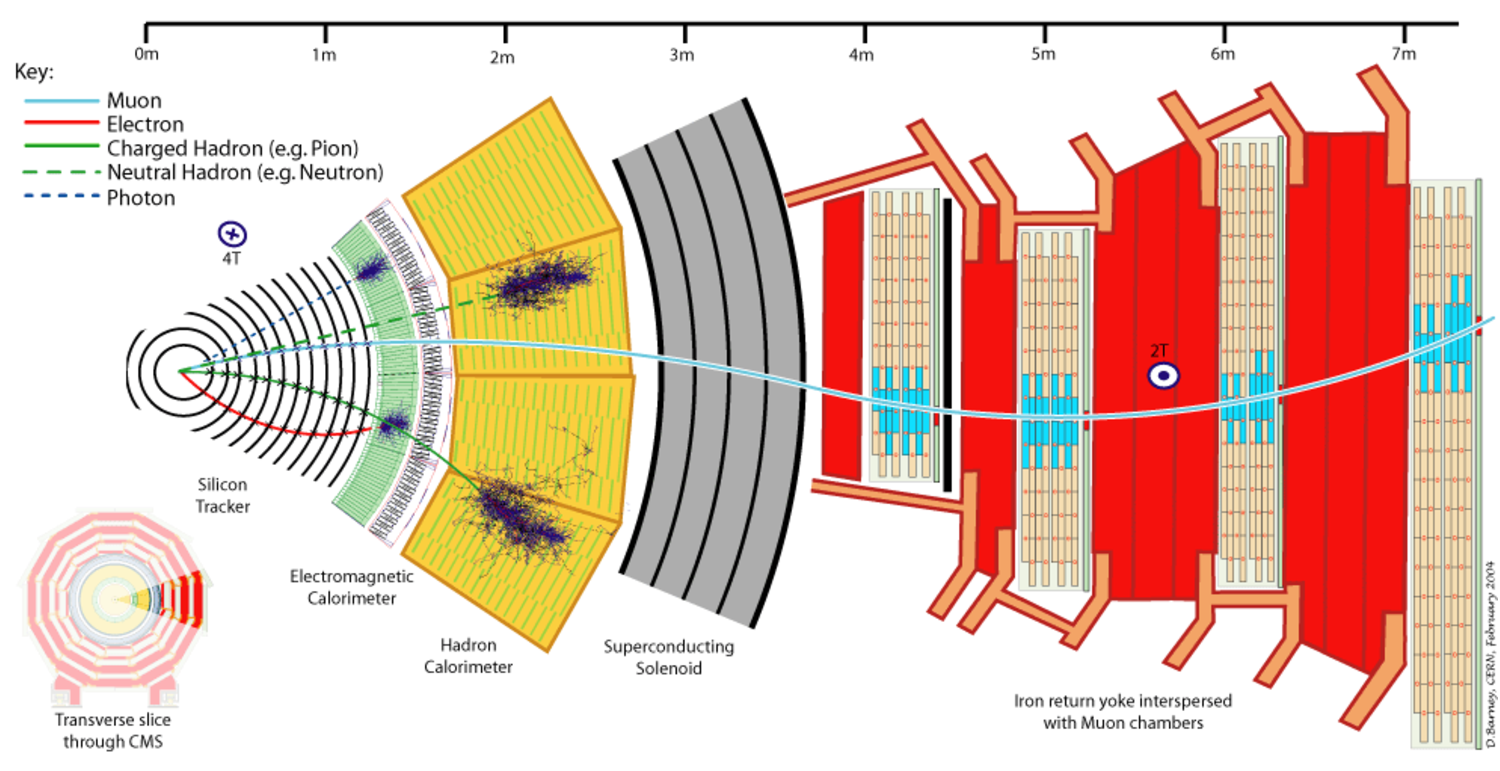
\includegraphics[width=\linewidth]{Figures/EventReconstruction/cms_slice.pdf}
       \caption{Slice of the transverse plane of the CMS detector showing how different particles interact with the detector sub-systems. The most important particle for this analysis is the photon (blue dotted line), which interacts only with the ECAL (shown in green).
       Reprinted from Reference~\cite{CDS}.}
       \label{fig:cmsSlice}
\end{figure*}

Of course, the simplified picture in Figure~\ref{fig:cmsSlice} does not cover the full complexity of how particles can interact with the detector. Photons can ``convert" and produce an electron-positron pair. Hadrons can interact with the material of the tracker or ECAL, and begin to shower before reaching the HCAL. The following sections will describe in more detail how physics objects are reconstructed. 

\subsection{Photons}
\label{sec:phoReco}
%https://www3.nd.edu/~cjessop/talks/JessopCMS101.pdf

\subsection{Electrons}
\label{sec:eleReco}

Describe how tracks are reconstructed

\subsection{Particle Flow Algorithm}
\label{sec:ParticleFlow}
Objects that go into the jet clustering algorithm are reconstructed using PF \cite{ParticleFlow}.

\subsection{Jet reconstruction}
\label{sec:Jet}
Jets are reconstructed using the \antikt algorithm with a distance parameter of $R <$ 0.4~\cite{antikt}.  The \antikt algorithm is a sequential clustering algorithm where the distance $d_{ij}$ between two particles $i$ and $j$ and the distance $d_{iB}$ between particle $i$ and the beam $B$ is given by the following: 
\begin{equation}
d_{ij} = \mathrm{min}(k_{ti}^{2p},k_{ti}^{2p})\frac{\Delta^2_{ij}}{R^2},
d_{iB} =k_{ti}^{2p}
\end{equation}
The value $\Delta^2_{ij}$ is equal to $(\eta_i - \eta_j)^2 + (\phi_i - \phi_j)^2$, $k_t$ is the transverse momentum of the particle, and $R$ is a distance parameter that determines the final radius of the jet.

The clustering algorithm first finds the smallest value of $d_{ij}$ and $d_{iB}$ for all particles in the event. If the minimum distance is $d_{ij}$, then particles $i$ and $j$ are combined into a single entity. If the minimum distance is $d_{iB}$, then particle $i$ is labelled a jet and removed from the list. For the \antikt algorithm, the parameter $p = -1$. Setting $p=0$ corresponds to the inclusive Cambridge/Aachen algorithm, and $p=1$ is the inclusive $k_t$ algorithm. The result of various jet-clustering algorithms is shown in Figure~\ref{fig:jetAlgorithms}.
 
 \begin{figure*}[h!]
	\centering
	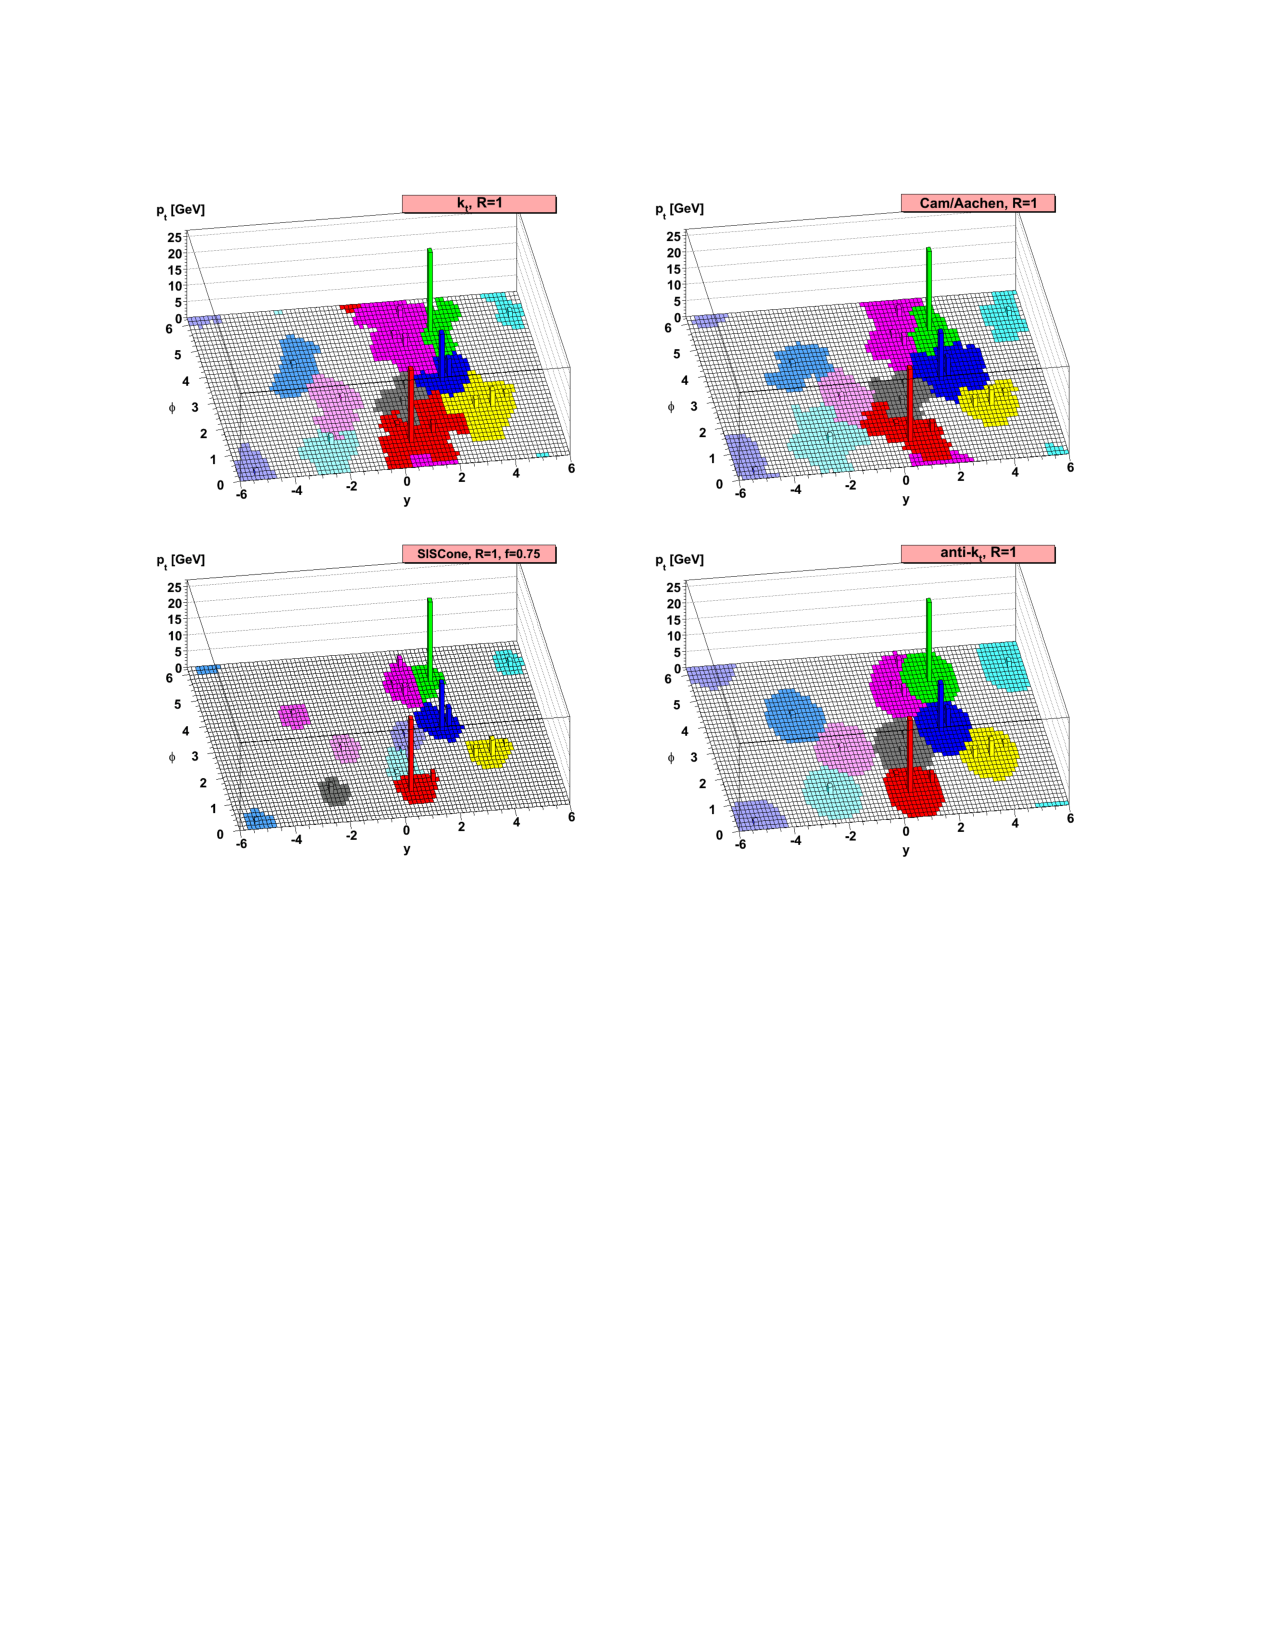
\includegraphics[width=\linewidth]{Figures/EventReconstruction/jetAlgorithms.pdf}
       \caption{Behavior of several jet-clustering algorithms illustrated with a sample parton-level event. 
       CMS uses the \antikt algorithm (bottom right) with a distance parameter $R = 0.4$.
       Reprinted from Reference~\cite{antikt}.}
       \label{fig:jetAlgorithms}
\end{figure*}
 
One benefit of the \antikt algorithm is that it is infrared and collinear (IRC) safe. Infrared safe means that \antikt jets are insensitive to nearby soft particles. In the \antikt algorithm, soft particles (those with $k_t \rightarrow 0$) have a large $d_{ij}$ and are therefore clustered last. This leaves hard jets unaffected. Soft particles could possibly by clustered into many soft jets, but those are simple to remove during the analysis. This is particularly important for the high luminosity environment of the LHC, because soft particles from pileup interactions will not change the clustering of the hard jets from the primary interaction. 

Collinear safe means that very energetic initial quarks will still get reconstructed as a single jet. In the \antikt algorithm, collinear particles will have a small value of $\Delta^2_{ij}$ and will be clustered together first. Using an IRC safe algorithm is important for comparing theory and experiment, because if jets are not IRC safe, then their cross sections cannot be calculated using perturbation theory.

\subsection{Pileup subtraction}
\label{}

